\chapter{Automates à pile}
	\section{Introduction}
	Quelque soit le langage et la classe du langage, celui-ci est reconnu par un automate est il est engendré par une grammaire.

	\begin{description}
		\item[Régulier] S'exprime avec une expression régulière et engendre un automate fini déterministe et est associé à une grammaire linéaire à
			droite. \\
			Langage régulier $\Longleftrightarrow$ Expression régulière $\Longleftrightarrow$ Automate fini déterministe $\Longleftrightarrow$ système d'équation de
			langage $\Longleftrightarrow$ Grammaire linéaire
		\item[Langage hors contexte] Ce sont les langages ayant besoin d'une mémoire, ils sont reconnus par un automate à pile et engendré par une grammaire hors contexte.
			\begin{exemple}
				Par exemple le langage $a^nb^n n\geq 0$ est un langage hors contexte. Il nécessite de connaître le nombre de a pour pouvoir faire les b.
				Sa grammaire hors contexte serait : 
				\begin{eqnarray*}
					S &\rightarrow& a S b\\
					S &\rightarrow& \lambda
				\end{eqnarray*}
			\end{exemple}

	\end{description}
	\section{Définition}
		\subsection{Informelle}\label{defInformelle}
			Un automate à pile possède le même fonctionnement d'un automate fini avec en plus une pile permettant de sauvegarder de l'information. 

		\begin{figure}[H]
			\centering
			\includegraphics[width=8cm]{autoPile.eps}
			\caption{Schéma d'un automate à pile}
			\label{fig:autoPile}
		\end{figure}
		\begin{remarque}
			Contrairement à un automate finis, un automate à pile peut lire $\lambda$ sur le ruban.~\\
		\end{remarque}
		\subsection{Formelle}
		Un automate à pile est un 7-uplet $<Q,X,F,\Gamma,q_0,Z_0,\delta>$
		\begin{itemize}
			\item $Q$ un ensemble finis d'états
			\item $X$ l'alphabet, un ensemble finis de symboles avec $\lambda \not\in X$
			\item $F$ un ensemble finis d'états finals avec $F \subset Q$, éventuellement $F=\varnothing$
			\item $\Gamma$ un ensemble fini de symboles de pile, éventuellement $\Gamma \cap X = \varnothing$
			\item $q_0 \in Q$, état initial
			\item $Z_0 \in Gamma$ symbole de fond de pile
			\item $\delta$: $Q \times (X \cup\{\lambda\})\times\Gamma\footnote{Un seule symbole $\in \Gamma$} \rightarrow P(Q\times\Gamma^*\footnote{Un
				mot à la plae du sommet de pile})$
		\end{itemize}

		\begin{attention}
			\begin{itemize}
				\item On peut accéder uniquement au sommet de pile
				\item On remplace le sommet de pile Z par un mot de $\lambda^*$
				\item Une pile qui contient $Z_0$ n'est pas vide
			\end{itemize}
		\end{attention}
	\section{Configuration}
	\subsection{Définition}
	Une configuration est une << photo de la machine >> à un instant donné, celle-ci est un triplet : L'état, le ruban et la pile, $(q, w, \gamma)$
	\begin{itemize}
		\item $q\in Q$
		\item $w \in X^*$
		\item $\gamma \in \Gamma$
	\end{itemize}

	Les lettres sont positionnées sur la figure \ref{fig:autoPile}.

	\subsection{Relation entre deux configuration}
	Soit deux configurations $(q,xu,Z\gamma)$ et $(q',u,\beta\gamma)$

	\begin{itemize}
		\item $q,q\in Q$
		\item $x \in X \cup\{\lambda\}$
		\item $Z \in \Gamma, \gamma \in\Gamma^*\beta \in\Gamma^*$
	\end{itemize}

\begin{definition}
	La relation $\leftharpoondown$ est la dérivation en une étape de calcul ($\delta$ si $\delta(q,x,Z)$ contient $(q,xu,Zj) \leftharpoondown (q',u\beta
	\gamma)$
\end{definition}

\begin{definition}
	La relation $\leftharpoondown^*$ exprime l'enchainement des étape de calcul.
\end{definition}

\subsection{Reconnaissance}
Triplet $(q_0,w,Z_0)$. Langage reconnu par un automate à pile A deux modes de reconnaissance.
\begin{description}
	\item[Par état final]$T(A) = \{w\in X^*/(q_0,w,Z_0)\leftharpoondown^*(qf,\lambda,\gamma)$ avec $qf _in F$
	\item[Par pile vide] $N(A) = \{w\in X^*/(q_0,w,Z_0)\leftharpoondown^*(q,\lambda,\lambda),q \in Q$
\end{description}

Deux modes de reconnaissance équivalents sont automatiquement à pile non déterministe.
	
\begin{exemple}
	Soit le langage $L=a^nb^n n\geq0$. Construire un automate à pile $A$ qui reconnait $L$

	Reconnaissance par pile vide.

	$A=<Q,X,F,\Gamma,q_0,Z_0,\delta>$
	\begin{itemize}
		\item $Q=\{q_0,$
		\item $X=\{a,b\}$
		\item $F=\varnothing$
		\item $\Gamma=\{Z_0,A$
	\end{itemize}
	\begin{lstlisting}[language=algo, numbers=none, framerule=0pt]
tantque on lit 'a' faire empiler 'A' fin tantque;
tantque on lit 'b' avec 'A' au sommet faire depiler fin tantque;
Le mot est reconnu, si quand on a fini de lire on retrouver $Z_0$ dans la pile 
\end{lstlisting}

\begin{itemize}
	\item $\delta : Q\times X\cup\{\lambda\}\times\Gamma \rightarrow P(Q,\Gamma^*)$\\
	\item $\delta(q_0,a,Z_0) = (q_0,AZ_0)$ on empile le premier 'a' lu 
	\item $\delta(q_0,a,A) = (q_0,AA)$ On empile tous les 'a' lus
	\item $\delta(q_0,b,A) = (q_1,\lambda)$ On dépile A au 1er'b' lu (dépiler = empiler $\lambda$)
	\item $\delta(q_1,b,A) = (q_1,\lambda)$ Dépiler A tant qu'on lit 'b'
	\item $\delta(q_1,\lambda,Z_0) = (q_1,\lambda)$ le mot est reconnu donc on vide la pile 
\end{itemize}
\end{exemple}
%	\section{Langages reconnu}
	\section{Déterminisme}
	Le déterminisme avec un automate à pile est le même principe qu'avec un automate fini.

	Un automate à pile est déterministe si 
	\begin{displaymath}
		\left.\begin{array}{c}
			\forall q \in Q\\
			\forall Z \in \Gamma\\
			\forall x \in X
		\end{array}\right)
		\begin{array}{c}
		Card(\delta(q,x,Z)) \leq 1\ et\ card(\delta(q,\lambda,Z)) = 0\\
		Ou\ Card(\delta(q,\lambda,Z)) \leq\ 1\ et\ card(\delta(q,x,Z)) = 0
		\end{array}
	\end{displaymath}

	\begin{remarque}
		Il existe des langages qu'on ne peut reconnaître qu'avec un automate à pile non déterministe.
	\end{remarque}

	\section{Automate à pile déduit d'une grammaire}
	\begin{itemize}
		\item Soit $L$ un langage hors contexte.
		\item Soit $G$ tel que $L(G) = L$
		\item $G= <N,X,P,S>$
		\item $P = \{B\rightarrow \alpha, B\in N \alpha \in(NUX)^*$
	\end{itemize}
	Il existe un automate à pile $A$ telque $L(A) = L(G) = L$ tel que
	\begin{itemize}
		\item La reocnnaissance se fait par pile vide $(F = \varnothing)$
		\item Il y a un seul était $Q=\{q\} ; q_0 = q\}$
		\item Non déterministe
	\end{itemize}

	Il simule toutes les tentatives de la grammaire pour engendrer un mot de $L(G) = L(A) = L$.

	\begin{eqnarray*}
		A &=&   <Q,X,F,\Gamma,q_0,Z_0,\delta>\\
		Q &=&  \{q\}\ ;\ q_0 =  q\ ;\ Z_0 = S\\
	F &=& \varnothing\ ;\ \Gamma = NUX\\
	\end{eqnarray*}
	\begin{displaymath}
		\delta\ tq 
		\left\{ \begin{array}{c}
			\delta(q,\lambda,) = \{(q,\alpha) \forall B \rightarrow \alpha P\}\\
			\delta(q,x,x) = (q,\lambda) \forall x \in X
		\end{array}\right.
	\end{displaymath}
